\documentclass[conference]{IEEEtran}
\IEEEoverridecommandlockouts

\usepackage[utf8]{inputenc}
\usepackage[T5,T1]{fontenc}   % T5 = Vietnamese glyphs; T1 stays the default
\usepackage{cite}
\usepackage{amsmath,amssymb}
\usepackage{graphicx}
\usepackage{booktabs}
\usepackage{multirow}
\usepackage{xcolor}
\usepackage{url}
\usepackage{pgfplots}
\pgfplotsset{compat=1.18}
\definecolor{c1}{HTML}{0D366B}\definecolor{c2}{HTML}{3987E5}\definecolor{c3}{HTML}{1BAF7A}
\definecolor{c4}{HTML}{EB6834}\definecolor{c5}{HTML}{6250D6}\definecolor{c6}{HTML}{C4314B}

% Vietnamese text in the T5 encoding, e.g. \vi{bạn}
\newcommand{\vi}[1]{{\fontencoding{T5}\selectfont #1}}
% Figure from Drive if it has been uploaded to figures/, otherwise a framed placeholder
\newcommand{\figorbox}[2]{%
  \IfFileExists{figures/#1}{\includegraphics[width=\linewidth]{figures/#1}}%
  {\fbox{\parbox[c][3.2cm][c]{0.92\linewidth}{\centering\small\texttt{\detokenize{#1}}\par\vspace{2pt}\footnotesize #2}}}}
\newcommand{\pp}{\,pp}

\begin{document}

\title{Reading Without Diacritics: How Open LLMs Lose, and Partly Recover, Vietnamese Understanding When Tone Marks Disappear}

\author{\IEEEauthorblockN{Anonymous Author(s)}
\IEEEauthorblockA{\textit{Affiliation withheld for review}}}

\maketitle

\begin{abstract}
Vietnamese is often typed without diacritics, yet diacritics mark tone and vowel quality: unaccented \textit{ban} may be \vi{\textit{bạn}} (friend), \vi{\textit{bán}} (sell) or \vi{\textit{bàn}} (table). We measure how much open large language models (LLMs) lose on such input, what predicts the loss, and what recovers it. We evaluate 19 instruction-tuned models (1.5--14B parameters, eight families) zero-shot on five Vietnamese tasks under seven noise conditions, with a validity gate fixed before any noisy result was examined. Removing all diacritics costs 41--67\% of a model's above-chance accuracy, depending on the task, and the loss grows monotonically with the share of stripped syllables. The loss is unchanged across four prompt templates, including English instructions (Spearman $\geq 0.95$ between model rankings), and shrinks by 0.086 per doubling of parameters, a trend that holds when three 14B models are added. Comparing models on the same noisy item, the one that finds the stripped input more surprising errs more often, also among models that share a tokenizer. Telling the model that the text may lack diacritics recovers none of the loss and re-estimating the calibration prior on the noisy inputs recovers 7\%, whereas restoring diacritics with an off-the-shelf restorer before prompting recovers 64\%. On 226 comments that their authors typed without diacritics, models score no better than on synthetically stripped comments, yet restoration does not help (+0.01 balanced accuracy, 95\% CI $[-0.02, 0.04]$). We release the noise suite, notebooks with built-in checks, and per-item predictions.
\end{abstract}

\begin{IEEEkeywords}
Vietnamese, diacritics, robustness, large language models, tokenization, diacritic restoration
\end{IEEEkeywords}

%=====================================================================
\section{Introduction}

Vietnamese uses diacritics for six tones and for several vowel qualities, so one unaccented string can stand for many words. Readers resolve the ambiguity from context, and many people type without diacritics in chat, comments and search queries: on keyboards without a Vietnamese input method, on mobile devices, or out of habit~\cite{naplava2018diacritics,nguyen2023visobert}. A model deployed on Vietnamese user text will see such input.

Earlier work showed that removing diacritics hurts fine-tuned Vietnamese encoders on social-media tasks~\cite{nguyen2023visobert} and zero-shot Vietnamese classifiers~\cite{ha2026decision}, where it was the most damaging of the perturbations tested. Practitioners, however, increasingly use open generative LLMs with a prompt and no fine-tuning, and for them four questions remain open:
\begin{enumerate}
\item \textbf{How much} is lost, and does it depend on the prompt, on the amount of noise and on model size?
\item \textbf{Who} is robust: larger models, or models adapted to Vietnamese?
\item \textbf{Why}: because unaccented text is tokenized differently, or because the model finds it surprising?
\item \textbf{What helps}: telling the model, or restoring the diacritics first? And does a fix measured on synthetic noise carry over to text people actually typed without diacritics?
\end{enumerate}

We answer them with 19 open LLMs of 1.5--14B parameters on five tasks. Our contributions are:
\begin{itemize}
\item A controlled measurement with full and partial diacritic removal, teen code and their mix, scored with single-token answers and a validity gate fixed in advance (\S\ref{sec:setup}--\ref{sec:effect}). The loss is monotone in the dose and does not depend on the prompt.
\item Evidence that the loss shrinks steadily with model size up to 14B, while Vietnamese-adapted models are not more robust (\S\ref{sec:who}).
\item A same-item analysis in which the increase in model surprise predicts errors even when tokenization is identical, together with a robust negative association of broken syllables that we report as unexplained (\S\ref{sec:why}).
\item A head-to-head comparison of mitigations on the same model--task pairs (a prompt hint, a noise-estimated calibration prior and automatic restoration), and a test on naturally unaccented comments (\S\ref{sec:fix}).
\end{itemize}

%=====================================================================
\section{Related Work}

\textbf{Vietnamese diacritics and robustness.}
ViSoBERT~\cite{nguyen2023visobert} removes 25--100\% of the diacritics from five Vietnamese social-media datasets and reports that all fine-tuned encoders, its own included, degrade, with smaller losses at lower removal rates. It attributes PhoBERT's larger loss to a tokenizer that cannot encode unaccented text. Ha et al.~\cite{ha2026decision} test four zero-shot ``decision models'' (an API model and three of 287--328M parameters) on 13 classification settings. Diacritic removal lowers mean macro-F1 by 9.5--15.5 points, against at most 1.1 for teen code and 4.5 for typos. Their LLM numbers are taken from earlier clean-input experiments~\cite{thin2024prompt} and are not re-run under noise. Neither study evaluates generative LLMs under diacritic removal, varies the prompt or model size, or compares mitigations. A recent benchmark tests LLMs on Vietnamese dialects~\cite{tran2026dialects} but not on diacritics. We extend this line to zero-shot generative LLMs and add size, prompt, mechanism and mitigation analyses. We also qualify the observation that teen code is harmless: in~\cite{ha2026decision}, teen code edits 2.1\% of characters against 18.3\% for diacritic removal, and at an equal dose the two do similar damage (\S\ref{sec:teencode}).

\textbf{Diacritics and tokenization.}
Tokenizers trained mostly on English split many other scripts and diacritized text into more tokens, which raises cost and can lower performance~\cite{rust2021tokenizer,petrov2023tokenizers}. Gorman and Pinter~\cite{gorman2024diacritics} argue that NLP pipelines should not strip or inconsistently encode diacritics. We test whether changes in tokenization explain the loss once item and model are held fixed.

\textbf{Diacritic restoration.}
Restoration is a well-studied sequence-labelling problem; Vietnamese is among the hardest languages for it~\cite{naplava2018diacritics}. Le-Hong~\cite{lehong2021diacritics} applies diacritic generation to hate speech detection on Vietnamese social networks. We evaluate an off-the-shelf restorer as a preprocessing defence for zero-shot LLMs and compare it with simply telling the model.

\textbf{Synthetic versus natural noise.}
Robustness to synthetic noise need not transfer to natural noise~\cite{belinkov2018noise}. We therefore also test restoration on comments that their authors typed without diacritics. Our protocol follows perturbation-based behavioural testing~\cite{ribeiro2020checklist}.

%=====================================================================
\section{Experimental Setup}\label{sec:setup}

\subsection{Tasks and items}
Table~\ref{tab:tasks} lists the five public tasks~\cite{nguyen2018vsfc,ho2019vsmec,luu2021vihsd,conneau2018xnli,nguyen2020vimmrc}. Test items come from the test split. Dev items, used only to choose the answer format and the calibration prior, come from the disjoint validation split. We apply NFC normalisation and remove duplicates, items with conflicting labels, items under three syllables and items with no diacritic. We then sample a balanced number of items per class, 1,835 test items in total. Noise is applied to the input fields only; the instruction and the answer options stay clean.

\begin{table}[t]
\centering
\caption{Tasks and test items (balanced per class).}
\label{tab:tasks}
\begin{tabular}{@{}llrr@{}}
\toprule
Task & Type & Classes & Items \\
\midrule
UIT-VSFC~\cite{nguyen2018vsfc} & student-feedback sentiment & 3 & 450 \\
UIT-VSMEC~\cite{ho2019vsmec} & social-media emotion & 7 & 245 \\
ViHSD~\cite{luu2021vihsd} & social-media hate speech & 3 & 450 \\
XNLI-vi~\cite{conneau2018xnli} & natural language inference & 3 & 450 \\
ViMMRC~\cite{nguyen2020vimmrc} & multiple-choice reading & 4 & 240 \\
\midrule
Total & & & 1,835 \\
\bottomrule
\end{tabular}
\end{table}

\subsection{Noise conditions}
\begin{itemize}
\item \texttt{clean}: the original text.
\item \texttt{partial25/50/75}: an exact share of the syllables that carry diacritics is stripped, drawn with three random seeds.
\item \texttt{strip}: all diacritics are removed (NFD decomposition, combining marks dropped, \vi{đ}$\rightarrow$d).
\item \texttt{teencode}: a hand-written substitution table (e.g.\ \vi{không}$\rightarrow$ko, \vi{được}$\rightarrow$dc); it changes 6--12\% of words.
\item \texttt{mixed}: teen code, then 50\% stripping.
\end{itemize}
Automatic checks stop the run if \texttt{strip} leaves a diacritic, if \texttt{partial} changes anything besides diacritics, or if the noise is not deterministic.

\subsection{Models}
We evaluate 19 instruction-tuned models (Table~\ref{tab:models}). Several families come in more than one size with the same tokenizer, which allows size comparisons with the tokenizer held fixed. Qwen2.5, Qwen3 and SeaLLMs-v3 share one tokenizer vocabulary, which gives a natural control for tokenization. Four models are adapted to Vietnamese or Southeast Asian languages by continued training: SeaLLMs-v3, released before Qwen2.5 and built on the Qwen2 architecture, and VinaLLaMA, built on Llama-2~\cite{nguyen2023vinallama}. The 14B models ran on one A100 80\,GB GPU and the others on one L4.

\begin{table}[t]
\centering
\caption{Models. VI: adapted to Vietnamese or Southeast Asian languages.}
\label{tab:models}
\begin{tabular}{@{}lllc@{}}
\toprule
Family & Sizes (B) & Tokenizer & VI \\
\midrule
Qwen2.5-Instruct & 1.5, 3, 7, 14 & Qwen (shared) & \\
Qwen3 & 1.7, 4, 8, 14 & Qwen (shared) & \\
SeaLLMs-v3-Chat & 1.5, 7 & Qwen (shared) & \checkmark \\
VinaLLaMA-chat & 2.7, 7 & VinaLLaMA & \checkmark \\
BLOOMZ & 1.7, 3, 7.1 & BLOOM & \\
Phi-3.5-mini / phi-4 & 3.8 / 14 & Phi & \\
Mistral-Instruct-v0.3 & 7 & Mistral & \\
Llama-3.2-Instruct & 3 & Llama-3 & \\
\bottomrule
\end{tabular}
\end{table}

\subsection{Prompting and scoring}
Each model receives its documented chat format; for Qwen3 the thinking mode is disabled (\texttt{enable\_thinking=False}). Options are presented as letters, and the answer is prefilled with \vi{``Đáp án:''} (``Answer:'') after the template's assistant header. For every model we check that each option letter is a single, distinct token. We read the probability of each letter from one forward pass, which also yields the summed negative log-likelihood (NLL) of the input fields. We normalise it by the number of syllables of the \emph{clean} input, so that $\Delta$NLL does not depend on how many tokens a tokenizer produces (\S\ref{sec:why}). The main predictions use batch calibration~\cite{zhou2024batch} with a prior estimated on clean dev items. Raw predictions are kept and lead to the same conclusions (\S\ref{sec:prompts}).

\subsection{Validity gate}
Before examining any noisy result, we fixed three conditions that a (model, task) pair must meet to be analysed:
\begin{itemize}
\item median probability mass on the option letters $\geq 0.5$;
\item agreement between a free greedy answer and the scored answer $\geq 0.7$, on 40 clean and 40 stripped items;
\item clean accuracy $\geq$ chance $+\,0.10$, with the lower bound of its 95\% CI above chance.
\end{itemize}
For the 16 models up to 8B, 74 of 80 pairs pass. The six exclusions all have clean accuracy near chance: five on ViHSD and BLOOMZ-1.7B on XNLI. The three 14B models pass on all five tasks, so 89 pairs are analysed in total.

\subsection{Metrics and statistics}
The \emph{normalised drop} under condition $c$ is
\begin{equation}
d_c = \frac{\mathrm{acc}_{\text{clean}} - \mathrm{acc}_c}{\mathrm{acc}_{\text{clean}} - \text{chance}},
\end{equation}
which is 0 for no loss and 1 for a fall to chance. For restoration we report the \emph{recovery}
\begin{equation}
r = \frac{\mathrm{acc}_{\text{restored}} - \mathrm{acc}_{\text{strip}}}{\mathrm{acc}_{\text{clean}} - \mathrm{acc}_{\text{strip}}},
\end{equation}
computed when the strip loss exceeds 0.05. CIs are 95\% paired bootstrap intervals over items ($B = 2000$, with the same resamples for every condition). Within-family tests use Holm correction. Regressions use fixed effects as stated, with standard errors clustered by item (\S\ref{sec:why}) or by model (\S\ref{sec:who}).

%=====================================================================
\section{How Much Is Lost?}\label{sec:effect}

\subsection{Full removal}
Table~\ref{tab:strip} shows the normalised drop under \texttt{strip}. A typical model loses between two fifths and two thirds of its above-chance accuracy. Reading comprehension (ViMMRC) loses least. Its long passages may give more context for resolving ambiguous words, but we have not tested this.

\begin{table}[t]
\centering
\caption{Mean normalised drop over valid models up to 8B, and the effect of automatic restoration (\S\ref{sec:fix}). Word acc.: share of words the restorer gets right.}
\label{tab:strip}
\setlength{\tabcolsep}{4pt}
\begin{tabular}{@{}lccccc@{}}
\toprule
& \multicolumn{2}{c}{\texttt{strip}} & \multicolumn{3}{c}{\texttt{restored}} \\
\cmidrule(lr){2-3}\cmidrule(l){4-6}
Task & $d$ [95\% CI] & $n$ & Word acc. & $d$ & Recovery [95\% CI] \\
\midrule
VSFC   & 0.67 [0.61, 0.74] & 16 & 92.5\% & 0.12 & 0.77 [0.68, 0.85] \\
VSMEC  & 0.66 [0.55, 0.76] & 16 & 76.2\% & 0.23 & 0.64 [0.50, 0.78] \\
XNLI   & 0.56 [0.45, 0.64] & 15 & 92.0\% & 0.10 & 0.73 [0.62, 0.87] \\
ViHSD  & 0.53 [0.44, 0.63] & 11 & 75.1\% & 0.24 & 0.52 [0.32, 0.66] \\
ViMMRC & 0.41 [0.36, 0.46] & 16 & 81.2\% & 0.15 & 0.55 [0.40, 0.67] \\
\bottomrule
\end{tabular}
\end{table}

\subsection{Dose-response}
Accuracy falls monotonically with the share of stripped syllables in 86\% of valid pairs with one noise seed. With accuracies averaged over three seeds, it falls monotonically in 97\%. The normalised drop differs by 0.048 between seeds on average (at most 0.121). There is no threshold below which removal is harmless (Fig.~\ref{fig:dose}). This agrees with the trend that ViSoBERT~\cite{nguyen2023visobert} reports for fine-tuned encoders.

\begin{figure}[t]
\centering
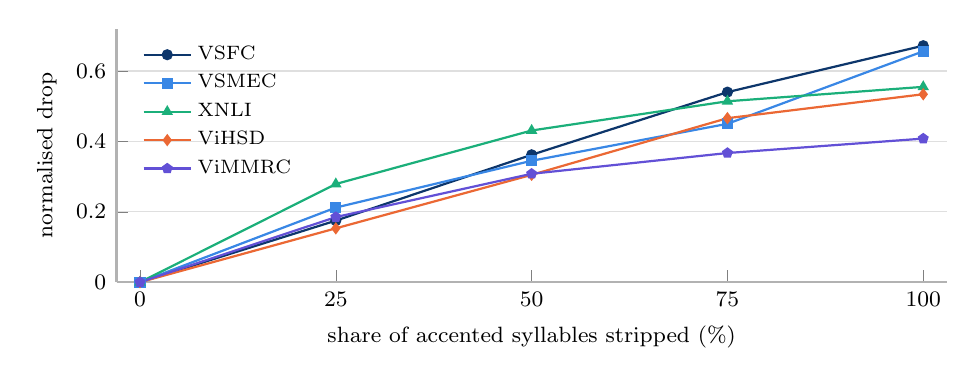
\begin{tikzpicture}
\begin{axis}[
  width=\linewidth, height=4.8cm, xmin=-3, xmax=103, ymin=0, ymax=0.72,
  xtick={0,25,50,75,100}, xlabel={share of accented syllables stripped (\%)}, ylabel={normalised drop},
  label style={font=\footnotesize}, tick label style={font=\footnotesize},
  legend style={font=\scriptsize, at={(0.02,0.98)}, anchor=north west, draw=none, fill=none},
  legend cell align=left, axis x line*=bottom, axis y line*=left,
  ymajorgrids, grid style={gray!25}, axis line style={gray!60}, mark size=1.6pt, thick,
]
\addplot[color=c1, mark=*] coordinates {(0,0) (25,0.175) (50,0.362) (75,0.540) (100,0.672)};
\addplot[color=c2, mark=square*] coordinates {(0,0) (25,0.212) (50,0.345) (75,0.450) (100,0.656)};
\addplot[color=c3, mark=triangle*] coordinates {(0,0) (25,0.279) (50,0.431) (75,0.514) (100,0.555)};
\addplot[color=c4, mark=diamond*] coordinates {(0,0) (25,0.153) (50,0.305) (75,0.466) (100,0.534)};
\addplot[color=c5, mark=pentagon*] coordinates {(0,0) (25,0.185) (50,0.308) (75,0.367) (100,0.408)};
\legend{VSFC, VSMEC, XNLI, ViHSD, ViMMRC}
\end{axis}
\end{tikzpicture}
\caption{Mean normalised drop over valid models up to 8B against the share of accented syllables stripped. Partial levels average three noise seeds; 100\% is \texttt{strip}. Seed-averaged 95\% CIs are about $\pm0.03$--$0.09$ and are omitted for legibility.}
\label{fig:dose}
\end{figure}

\subsection{Teen code is light, not harmless}\label{sec:teencode}
Teen code alone costs only 0.03--0.12 normalised drop per task (0.06 on average), against 0.33--0.47 for teen code followed by 50\% stripping. Our teen-code table, however, changes just 6--12\% of words. Partial diacritic removal at that same share of words does similar damage: 0.10 against 0.06 on VSFC and 0.11 against 0.12 on XNLI. The conclusion that teen code is harmless, here and in~\cite{ha2026decision}, should therefore be read as ``teen code as usually generated changes few words''.

\subsection{The loss does not depend on the prompt or the scoring}\label{sec:prompts}
We re-ran the clean and stripped conditions with three more templates: a Vietnamese paraphrase of the instruction; English instructions with the Vietnamese input unchanged; and the original template plus a sentence warning that the text may lack diacritics (``hint''). Table~\ref{tab:prompts} reports the 85 (model, task) pairs, including the 14B models, that are valid under all four templates; this is why its mean drop (0.52) differs from the 0.57 of the 74 pairs up to 8B. The mean drop varies by at most 0.03, and models rank almost identically. Only one task--template combination differs significantly from the original prompt: XNLI with English instructions (+0.07).

\begin{table}[t]
\centering
\caption{Mean normalised drop under \texttt{strip} for four prompt templates (85 pairs valid under all four), and Spearman correlation of the per-pair drops with those of the original template.}
\label{tab:prompts}
\begin{tabular}{@{}lcc@{}}
\toprule
Template & $d$ [95\% CI] & Spearman \\
\midrule
Original (Vietnamese) & 0.52 [0.48, 0.55] & --- \\
Vietnamese paraphrase & 0.52 [0.49, 0.56] & 0.96 \\
English instructions  & 0.55 [0.51, 0.58] & 0.95 \\
Original + hint       & 0.52 [0.48, 0.56] & 0.98 \\
\bottomrule
\end{tabular}
\end{table}

The result is also stable across scoring choices. Over the 74 valid pairs of the models up to 8B (Table~\ref{tab:strip}), the mean drop under \texttt{strip} is 0.57 with calibration, 0.59 without, 0.71 in macro-F1, and 0.53 when the model's free-text answer is parsed instead of scored. Keeping the six pairs excluded by the gate changes little (ViHSD 0.53$\rightarrow$0.59), and so does restricting the analysis to the 11 models valid on every task.

\subsection{What the errors look like}
Probability mass on the option letters barely changes under \texttt{strip}, so models still answer in the expected format: the errors are changes of judgement. Predictions do drift toward one label: under \texttt{strip}, the most frequent predicted label takes more than 60\% of the predictions in 27 of 74 valid pairs (on VSFC, seven models drift toward \textit{negative}). \S\ref{sec:prior} tests whether re-estimating the calibration prior on the noisy inputs undoes this.

%=====================================================================
\section{Who Is Robust?}\label{sec:who}

\textbf{Size.} We regress the \texttt{strip} drop of each valid pair on $\log_2$(parameters), with task and family fixed effects and standard errors clustered by model. Because there are only 11--19 clusters, Table~\ref{tab:inference} reports $p$-values from a $t$ distribution with $G-1$ degrees of freedom and from a restricted wild cluster bootstrap (Webb weights, 9,999 draws), not from the normal approximation. The drop shrinks by 0.090 per doubling across the 16 models up to 8B, and by 0.086 [$-0.104$, $-0.068$] when the three 14B models are added (wild bootstrap $p = 0.001$; 19 models, 89 pairs). With family fixed effects, families with a single model (Mistral, Llama-3.2, Phi-3.5, phi-4) do not inform the slope, so the Phi-3.5$\rightarrow$phi-4 change of generation cannot drive it; dropping both Phi models or keeping only the three families with at least three sizes leaves the slope at $-0.086$ and $-0.093$. The 14B models lose 0.24 (Qwen3-14B), 0.30 (Qwen2.5-14B) and 0.44 (phi-4) on average. Size helps, but even the most robust 14B model still loses about a quarter of its above-chance accuracy. Pairwise tests within a family have less power: the largest model is significantly more robust than the smallest in only 5 of 22 family--task tests after Holm correction, four of them on VSFC (e.g.\ Qwen2.5, 0.73$\rightarrow$0.27; Qwen3, 0.55$\rightarrow$0.17).

\begin{figure}[t]
\centering
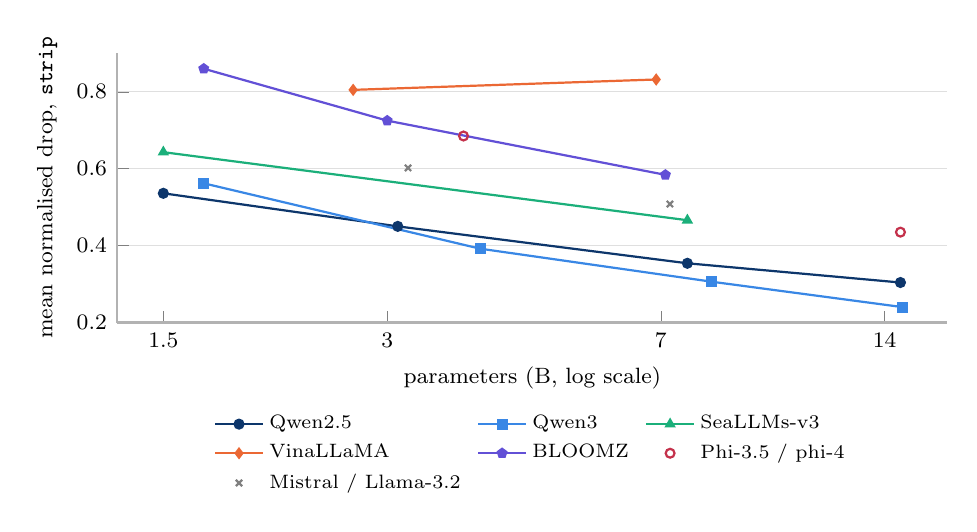
\begin{tikzpicture}
\begin{axis}[
  width=\linewidth, height=5cm, xmode=log, log basis x=2, xmin=1.3, xmax=17, ymin=0.2, ymax=0.9,
  xtick={1.5,3,7,14}, xticklabels={1.5,3,7,14}, xlabel={parameters (B, log scale)}, ylabel={mean normalised drop, \texttt{strip}},
  label style={font=\footnotesize}, tick label style={font=\footnotesize},
  legend style={font=\scriptsize, at={(0.5,-0.3)}, anchor=north, draw=none, fill=none, legend columns=3, /tikz/every even column/.append style={column sep=4pt}},
  legend cell align=left, axis x line*=bottom, axis y line*=left,
  ymajorgrids, grid style={gray!25}, axis line style={gray!60}, mark size=1.6pt, thick,
]
\addplot[color=c1, mark=*] coordinates {(1.5,0.536) (3.1,0.450) (7.6,0.354) (14.7,0.304)};
\addplot[color=c2, mark=square*] coordinates {(1.7,0.562) (4.0,0.392) (8.2,0.306) (14.8,0.240)};
\addplot[color=c3, mark=triangle*] coordinates {(1.5,0.643) (7.6,0.466)};
\addplot[color=c4, mark=diamond*] coordinates {(2.7,0.805) (6.9,0.832)};
\addplot[color=c5, mark=pentagon*] coordinates {(1.7,0.860) (3.0,0.725) (7.1,0.584)};
\addplot[color=c6, only marks, mark=o] coordinates {(3.8,0.685) (14.7,0.435)};
\addplot[color=gray, only marks, mark=x] coordinates {(7.2,0.508) (3.2,0.602)};
\legend{Qwen2.5, Qwen3, SeaLLMs-v3, VinaLLaMA, BLOOMZ, Phi-3.5 / phi-4, Mistral / Llama-3.2}
\end{axis}
\end{tikzpicture}
\caption{Mean normalised drop under \texttt{strip} over each model's valid tasks against size (log scale); lines join sizes of one family. Models up to 8B from the main run, 14B models from the extension run.}
\label{fig:size}
\end{figure}

\begin{table}[t]
\centering
\caption{Inference with few clusters (clusters = models). Coefficient with a $t(G-1)$ 95\% CI; $p$-values from the normal approximation, $t(G-1)$, and a restricted wild cluster bootstrap.}
\label{tab:inference}
\footnotesize
\setlength{\tabcolsep}{2.5pt}
\begin{tabular}{@{}lccccc@{}}
\toprule
Sample & Coef. [95\% CI] & $p_{\mathcal N}$ & $p_t$ & $p_{\text{wild}}$ & $G$ \\
\midrule
\multicolumn{6}{@{}l}{\emph{Size: drop per doubling of parameters}} \\
Up to 8B & $-0.090$ [$-0.11$, $-0.07$] & $6{\cdot}10^{-16}$ & $8{\cdot}10^{-7}$ & 0.003 & 16 \\
With 14B & $-0.086$ [$-0.10$, $-0.07$] & $1{\cdot}10^{-22}$ & $1{\cdot}10^{-8}$ & 0.001 & 19 \\
No Phi models & $-0.086$ [$-0.10$, $-0.07$] & $5{\cdot}10^{-23}$ & $3{\cdot}10^{-8}$ & 0.001 & 17 \\
$\geq$3 sizes only & $-0.093$ [$-0.12$, $-0.07$] & $3{\cdot}10^{-20}$ & $3{\cdot}10^{-6}$ & 0.003 & 11 \\
\midrule
\multicolumn{6}{@{}l}{\emph{Adapted minus general (size and task controlled)}} \\
Up to 8B & $+0.159$ [$-0.04$, $+0.36$] & 0.086 & 0.11 & 0.16 & 16 \\
With 14B & $+0.169$ [$-0.03$, $+0.37$] & 0.072 & 0.089 & 0.14 & 19 \\
\bottomrule
\end{tabular}
\end{table}

\textbf{Vietnamese adaptation: no evidence of more robustness.} With size and task controlled, the four adapted models (SeaLLMs-v3 1.5B/7B, VinaLLaMA 2.7B/7B) lose 0.16 [$-0.04$, 0.36] \emph{more} than general models, which is not significant (wild bootstrap $p = 0.16$, Table~\ref{tab:inference}). This comparison mixes adaptation with the base model: SeaLLMs-v3 continues Qwen2, not the newer Qwen2.5 it shares a vocabulary with, and VinaLLaMA's Llama-2 base is not in our suite. We therefore read it as descriptive. SeaLLMs-v3 loses more than Qwen2.5 of the same size in 8 of 9 task comparisons (only VSFC survives Holm correction), and adapted models show a larger NLL increase under \texttt{strip} (2.96 vs.\ 1.71 nats per clean syllable); one possible reason is continued pre-training on edited, fully accented text, which we do not test here.

%=====================================================================
\section{What Predicts Errors?}\label{sec:why}

For each noisy item that a model answered correctly when clean, we model whether it now errs (a \emph{flip}) with a linear probability model. The main specification has item$\times$condition and model fixed effects, so it compares different models on the same noisy item; standard errors are clustered by item. Its predictors vary across models: the standardised clean-to-noisy changes in
\begin{itemize}
\item NLL of the input fields per clean syllable ($\Delta$NLL);
\item tokens per syllable ($\Delta$tokens);
\item share of syllables split across tokens ($\Delta$broken).
\end{itemize}
The ambiguity of the stripped words (the number of their accented readings, in bits) is a property of the item, identical for every model, so the item$\times$condition effects absorb it. We estimate it in a separate model with model, task and condition fixed effects instead (Table~\ref{tab:why}, panel C). All estimates are associations; none of them identifies a cause.

\begin{table}[t]
\centering
\caption{Linear probability models of flips: change in flip probability per SD of each predictor (percentage points, 95\% CI). Each panel is a separate regression.}
\label{tab:why}
\setlength{\tabcolsep}{4pt}
\begin{tabular}{@{}lcc@{}}
\toprule
Predictor & Effect (pp/SD) & $p$ \\
\midrule
\multicolumn{3}{@{}l}{\emph{A. Same item: item$\times$condition + model FE, all models up to 8B}} \\
$\Delta$NLL & +1.8 [1.0, 2.6] & $2.5\times10^{-5}$ \\
$\Delta$tokens & +2.6 [1.2, 4.0] & $3.9\times10^{-4}$ \\
$\Delta$broken & $-3.9$ [$-5.6$, $-2.2$] & $9.3\times10^{-6}$ \\
\multicolumn{3}{@{}l}{\emph{A$'$. As A, without Phi-3.5 and Mistral}} \\
$\Delta$NLL & +1.9 [1.0, 2.9] & $3.1\times10^{-5}$ \\
$\Delta$broken & $-6.3$ [$-9.3$, $-3.2$] & $5.4\times10^{-5}$ \\
\multicolumn{3}{@{}l}{\emph{B. Same item, Qwen2.5 / Qwen3 / SeaLLMs-v3 (one tokenizer)}} \\
$\Delta$NLL per clean syllable & +3.5 [2.4, 4.7] & $3\times10^{-9}$ \\
$\Delta$NLL per token & +3.7 [2.5, 4.9] & $2\times10^{-9}$ \\
\multicolumn{3}{@{}l}{\emph{C. Model + task + condition FE, partial and strip only}} \\
Ambiguity of stripped words & +2.0 & $1.6\times10^{-5}$ \\
$\Delta$NLL & +3.0 & $2.8\times10^{-9}$ \\
$\Delta$tokens & $-1.5$ & 0.014 \\
\bottomrule
\end{tabular}
\end{table}

\textbf{$\Delta$NLL predicts errors.} The model that finds a stripped item more surprising, relative to the clean version, is more likely to get it wrong (panel A). The association is twice as strong among Qwen2.5, Qwen3 and SeaLLMs-v3, whose tokenization of each item is identical (panel B), so it does not come from tokenization differences, and it is the same whether NLL is normalised per clean syllable or per token. $\Delta$NLL and flips may be two symptoms of one failure to reconstruct the meaning, so we do not read this as a mechanism. Across items, stripped words with more accented readings go with more flips (panel C).

\textbf{Tokenization measures pull in opposite directions.} $\Delta$tokens and $\Delta$broken are strongly correlated ($r = 0.87$) yet enter with opposite signs, and the same pattern appears at the model level ($\Delta$fertility $+0.145$, $p = 0.019$; $\Delta$broken $-0.192$, $p = 0.005$). Fragmentation therefore does not give a simple ``more pieces, more errors'' account. Phi-3.5 and Mistral even produce \emph{fewer} tokens after stripping and still lose heavily.

\textbf{An unexplained negative effect.} More broken syllables after stripping go with \emph{fewer} errors. We checked that this is not an artefact:
\begin{itemize}
\item \emph{Collinearity}: the variance inflation factor is about 4, and the sign holds when $\Delta$broken is entered alone ($-1.6$\pp, $p = 1.4\times10^{-4}$).
\item \emph{Clean tokenization}: the effect survives a control for the clean break rate ($-3.8$\pp, $p = 1.4\times10^{-5}$), which itself adds nothing ($p = 0.83$).
\item \emph{Subsamples}: it stays negative in all 14 leave-one-tokenizer-group and leave-one-family-out refits ($-4.6$ to $-2.3$\pp) and under another definition ($-4.1$\pp).
\item \emph{Direction of the tokenizer}: it is stronger, not weaker, when Phi-3.5 and Mistral, whose tokenizers split fewer syllables after stripping, are left out together ($-6.3$\pp; $-2.3$\pp entered alone; panel A$'$).
\end{itemize}
Tokenizers also differ in direction. Phi-3.5, Mistral and phi-4 split 80--90\% of clean Vietnamese syllables and \emph{fewer} after stripping (phi-4: 0.81$\rightarrow$0.50), while all other tokenizers split more. We report this effect as open and make no causal claim about broken syllables.

%=====================================================================
\section{Can It Be Fixed?}\label{sec:fix}

\subsection{A prompt hint does nothing}
Adding the sentence ``the text may be written without diacritics'' changes clean and stripped accuracy by less than one point on every task. It recovers $-1\%$ of the lost accuracy on average, and no task's CI excludes zero in its favour.

\subsection{Re-estimating the calibration prior helps little}\label{sec:prior}
Our main predictions divide by a prior estimated on clean dev items. A system that receives only unaccented input could instead estimate the prior on that input, without labels. Doing so on the stripped test inputs recovers 7\% [5, 10] of the lost accuracy over the 74 valid pairs up to 8B (mean drop 0.57$\rightarrow$0.52). It does reduce label collapse, from 27 to 14 pairs in which one label takes more than 60\% of the predictions, but most errors are not a shift of the label prior.

\subsection{Restoring diacritics recovers most of the loss}
We restore the stripped text with an off-the-shelf restorer, a token classifier fine-tuned from XLM-R large and released under Apache-2.0\footnote{\url{https://huggingface.co/peterhung/vietnamese-accent-marker-xlm-roberta}}, using 120-word windows, and score the result as before. Restoration recovers 64\% of the loss on average (65\% on the same 74 pairs as \S\ref{sec:prior}), and the remaining drop is 0.17 instead of 0.57 (Table~\ref{tab:strip}). On the 85 pairs of Table~\ref{tab:prompts} it recovers 60\% (49--71\% per task), while the hint recovers $-1\%$ (Fig.~\ref{fig:fix}).

\begin{figure}[t]
\centering
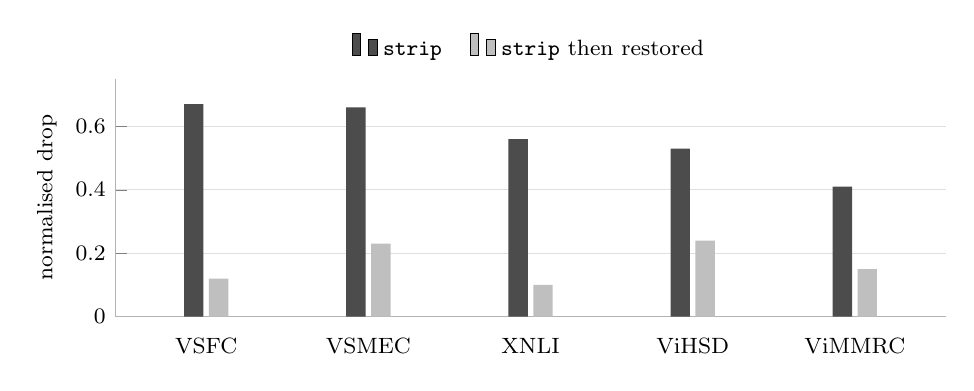
\begin{tikzpicture}
\begin{axis}[
  width=\linewidth, height=4.6cm,
  ybar, bar width=7pt, ymin=0, ymax=0.75,
  symbolic x coords={VSFC,VSMEC,XNLI,ViHSD,ViMMRC},
  xtick=data, ylabel={normalised drop},
  ylabel style={font=\footnotesize}, tick label style={font=\footnotesize},
  legend style={font=\footnotesize, at={(0.5,1.03)}, anchor=south, draw=none, fill=none, legend columns=2, /tikz/every even column/.append style={column sep=8pt}},
  axis x line*=bottom, axis y line*=left, xtick style={draw=none},
  legend cell align=left, enlarge x limits=0.14,
  ymajorgrids, grid style={gray!25}, axis line style={gray!60},
]
\addplot[fill=black!70, draw=none] coordinates {(VSFC,0.67) (VSMEC,0.66) (XNLI,0.56) (ViHSD,0.53) (ViMMRC,0.41)};
\addplot[fill=black!25, draw=none] coordinates {(VSFC,0.12) (VSMEC,0.23) (XNLI,0.10) (ViHSD,0.24) (ViMMRC,0.15)};
\legend{\texttt{strip}, \texttt{strip} then restored}
\end{axis}
\end{tikzpicture}
\caption{Mean normalised drop over valid models up to 8B, before and after automatic diacritic restoration. A prompt hint leaves the \texttt{strip} bars unchanged (recovery $-1\%$).}
\label{fig:fix}
\end{figure}

The benefit follows the restorer's accuracy. It is lower on the two social-media tasks, and not because their original text already lacks diacritics. Words that the original writes without diacritics where formal text uses them, together with slang and foreign words, make up only 4.5\% (VSMEC) and 5.7\% (ViHSD) of the words. Excluding them barely changes restoration accuracy (VSMEC 0.762$\rightarrow$0.775, ViHSD 0.751$\rightarrow$0.749). The restorer is simply weaker on informal text. Restoration also recovers less for the 14B models: 23\% (Qwen2.5-14B), 42\% (Qwen3-14B) and 50\% (phi-4). These models lose less to begin with, so restoration errors weigh relatively more: after restoration, 14 of their 15 valid pairs remain significantly below clean accuracy (by 9, 5 and 7 points on average). The restorer was trained on Vietnamese news titles, a domain distinct from our test sets, so we do not expect memorised test items, although without its training data we cannot exclude overlap.

\subsection{Naturally unaccented text}
Synthetic stripping removes every diacritic from text that was written with them, whereas people who type without diacritics may write differently. After the same cleaning as our test items, 270 ViHSD test comments contain no diacritic at all. We keep the 226 in which the restorer changes at least 20\% of the words (most of the other 44 are English, names or slang); on these, it adds diacritics to 70\% of the words. Over 14 valid models, restoration changes balanced accuracy by +0.01 [$-0.02$, 0.04], whereas the same models gain +0.055 on synthetic ViHSD items. Only VinaLLaMA-7B gains significantly (+0.17), and no model loses significantly.

Models do not read these comments well. Over the 14 models, mean balanced accuracy is 0.45 on the natural comments, the same as on our accented ViHSD test comments after stripping (0.45) and well below the same accented comments as written (0.56). On a scale where 0 is the stripped level and 1 the clean level, the median model sits at 0.12. The two sets contain different comments, so this is not a causal comparison, but it argues against the explanation that models already read habitual unaccented writing well. The remaining explanations are that the restorer fails on informal writing, or that these comments are harder for reasons unrelated to diacritics; a manually diacritized sample, in preparation, will separate them. The set is small and unbalanced (170 \textit{clean}, 15 \textit{offensive}, 41 \textit{hate}), so per-model CIs are wide. We read this as a caution rather than a negative result: gains measured on synthetic stripping should not be assumed for real unaccented input.

%=====================================================================
\section{Discussion}

Three points matter for practitioners. First, unaccented input can cost a model about half of its above-chance accuracy, and prompt changes, including telling the model, do not fix it. Second, larger models lose less, steadily up to 14B, but not to zero. Third, restoring diacritics is cheap and helps on stripped formal text, but its benefit should be checked on the target users' own writing before relying on it.

For research, the main open question is the gap between synthetic and natural unaccented text. Closing it needs a larger, balanced labelled corpus of naturally unaccented text and a restorer trained on informal writing. A training-side remedy is a hypothesis worth testing rather than a conclusion of this study: if adding unaccented text to continued pre-training lowers $\Delta$NLL, the association in \S\ref{sec:why} suggests, but does not establish, that the loss would shrink.

%=====================================================================
\section{Limitations}

\begin{itemize}
\item \emph{Scale}: the largest models have 14B parameters, and no closed model is tested; the size trend may flatten beyond 14B. Only two families (Qwen2.5, Qwen3) reach 14B; phi-4 differs from Phi-3.5 in generation and data as well as size, and with family fixed effects it does not inform the slope.
\item \emph{Restorer}: we use a single restorer, trained on Vietnamese news titles. Our test sets are not news titles, but overlap cannot be excluded without its training data. Its mean word accuracy on our data (83.4\%) is below the 85\% we set as a target in advance, so a better restorer may recover more.
\item \emph{Natural text}: the naturally unaccented set has 226 items from one task, selected with the restorer's output ($\geq$ 20\% of words changed).
\item \emph{Adaptation}: our adapted models are not compared with their exact base models (Qwen2, Llama-2).
\item \emph{Synthetic noise}: real unaccented writing is not uniformly random, since people may drop diacritics on frequent words first.
\item \emph{Answer format}: we score single-letter answers. This measures understanding, not generation; free-generation agreement is gated, but generation tasks are not covered.
\item \emph{Teen code}: the table is small and hand-written.
\item \emph{Mechanism}: all item-level results are associations; $\Delta$NLL and errors may share a cause, and the negative broken-syllable association is unexplained.
\end{itemize}

\section*{Ethics Statement}
We use public research datasets under their licences. ViHSD contains offensive content; we show no examples from it. Derived noisy datasets will be released only where the original licences allow.

\bibliographystyle{IEEEtran}
\bibliography{refs}

\end{document}
